% Lecture Template for ME3001 - Mechanical Engineering Analysis - Tennessee Technological University
% Spring 2024 - condensing and streamlining lectures by combining topics into a single PDF under the module name
% this will simplify file and link management as well as make lectures easier to use in class
% - added image/ to clean directory and reduce redundancy, specific to module for now  

% Module Name: - Non-Linear Equations
% Topic 1 - Solving Non-Linear Equations
% Topic 2 - The Newton-Raphson Method, Secant Method
% Topic 3 - The Bisection Method
% Topic 4 - Mechanical Design Problem

\documentclass[fleqn]{beamer} % for presentation (has nav buttons at bottom)

%\usepackage{/home/tntech.edu/thill/courses/dmc/lectures/dmc_lectures}
\usepackage{/home/thill/courses/analysis_lectures/lectures/analysis_lectures}
%\usepackage{/mnt/c/Users/thill/Documents/courses/analysis_lectures/lectures/analysis_lectures}

\author{ME3001 - Mechanical Engineering Analysis}

\newcommand{\MNUM}{1\hspace{2mm}} % module number 
\newcommand{\moduletitle}{Introduction and MATLAB Review}

\newcommand{\sectionItitle}{Solving Non-Linear Equations}
\newcommand{\sectionIItitle}{The Newton-Raphson Method, Secant Method}
\newcommand{\sectionIIItitle}{The Bisection Method}
\newcommand{\sectionIVtitle}{Mechanical Design Problem}

\newcommand{\sectionIsubsectionItitle}{What is a Non-Linear Equation ?}
\newcommand{\sectionIsubsectionIItitle}{Solving Non-linear Equations}
\newcommand{\sectionIsubsectionIIItitle}{Analytical vs. Numerical Methods}
\newcommand{\sectionIsubsectionIVtitle}{Example}

\newcommand{\sectionIIsubsectionItitle}{Classification of Methods}
\newcommand{\sectionIIsubsectionIItitle}{Taylor Series Derivation}
\newcommand{\sectionIIsubsectionIIItitle}{The Newton Raphson Method}
\newcommand{\sectionIIsubsectionIVtitle}{The Finite Difference}
\newcommand{\sectionIIsubsectionVtitle}{Modified Newton-Raphson, Secant Method}
\newcommand{\sectionIIsubsectionVItitle}{Algorithm Comparison}

\newcommand{\sectionIIIsubsectionItitle}{Analytical vs. Numerical}
\newcommand{\sectionIIIsubsectionIItitle}{A Bracketing Method: Graphical Explanation}
\newcommand{\sectionIIIsubsectionIIItitle}{Algorithm Description}
\newcommand{\sectionIIIsubsectionIVtitle}{Programming Exercise}

\newcommand{\sectionIVsubsectionItitle}{Problem Statement}
\newcommand{\sectionIVsubsectionIItitle}{Mathematical Model}
\newcommand{\sectionIVsubsectionIIItitle}{Solution Approach}
\newcommand{\sectionIVsubsectionIVtitle}{Design}

% custom box
\newsavebox{\mybox}

\title{Lecture Module - \moduletitle}

\date{Mechanical Engineering\vspc Tennessee Technological University}

\begin{document}

	\lstset{language=MATLAB,basicstyle=\ttfamily\small,showstringspaces=false}

	\frame{\titlepage \center\begin{framed}\Large \textbf{Module \MNUM - \moduletitle}\end{framed} \vspace{5mm}}

	% Module Outline
	\begin{frame} 
		\large \textbf{Module \MNUM - \moduletitle} \vspace{3mm}\\

		\begin{itemize}
			\item Topic 1 - \hyperlink{sectionI}{\sectionItitle} \vspc % section I
			\item Topic 2 - \hyperlink{sectionII}{\sectionIItitle} \vspc % section II
			\item Topic 3 - \hyperlink{sectionIII}{\sectionIIItitle} \vspc % section III
		\end{itemize}

	\end{frame}

	% section I
	\section{\sectionItitle}\label{sectionI}

		% section I Outline
		\begin{frame} 
			\large \textbf{Topic 1 - \sectionItitle} \vspace{3mm}\\

			\begin{itemize}
				\item \hyperlink{sectionIsubsectionI}{\sectionIsubsectionItitle} \vspc %  section I subsection I
				\item \hyperlink{sectionIsubsectionII}{\sectionIsubsectionIItitle} \vspc % section I subsection II
				\item \hyperlink{sectionIsubsectionIII}{\sectionIsubsectionIIItitle} \vspc % section I subsection III
				\item \hyperlink{sectionIsubsectionIV}{\sectionIsubsectionIVtitle} \vspc % section I subsection IV
			\end{itemize}
		\end{frame}
		
		% section I subsection I 
		\subsection{\sectionIsubsectionItitle}\label{sectionIsubsectionI}

			\begin{frame}
				\frametitle{\sectionIsubsectionItitle}
				\bigskip

				\textbf{Different Types of Non-Linear Equations }
		
				\begin{itemize}
					\item \textbf{Polynomials (excluding first order)} \vspace{3mm}
					\item \textbf{ Transcendentals} \vspace{2mm}

					{" a transcendental function "transcends" algebra in that it cannot be expressed in terms of a finite sequence of the algebraic operations of addition, multiplication, and root extraction. Examples of transcendental functions include the exponential function, the logarithm, and the trigonometric functions. "}\\
					\begin{itemize}
						\item Exponentials \vspace{1mm}
						\item Logarithms \vspace{1mm}
						\item Trigonometrics \vspace{2mm}
					\end{itemize}

				\end{itemize}

				\btVFill
			\end{frame}

			\begin{frame}
				\frametitle{\sectionIsubsectionItitle}
				\bigskip

				\btVFill
			\end{frame}

		% section I subsection II
		\subsection{\sectionIsubsectionIItitle}\label{sectionIsubsectionII}

			\begin{frame}
				\frametitle{\sectionIsubsectionIItitle}
				\bigskip

					\textbf{ Example:} Solve the following equation. \vspace{2mm} \\

					\hspace{2mm}\scalebox{1.0}{$y = x^2 + 2x - 10$}	 \vspace{2mm}

					\hspace*{-1cm}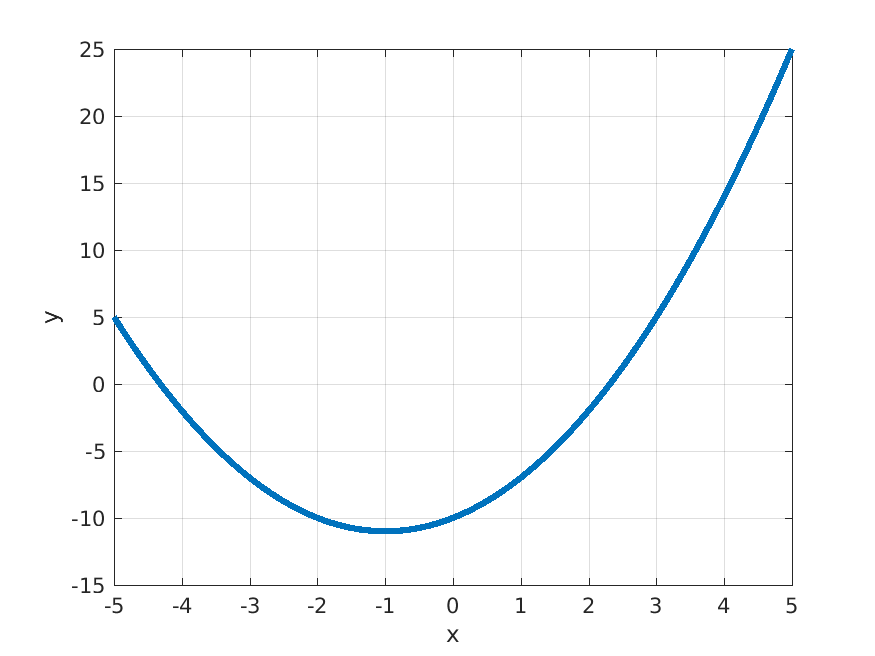
\includegraphics[scale=.45]{images/lecture1_fig1.png}  

				\btVFill
			\end{frame}

				%\btVFill
			\begin{frame}
				\frametitle{\sectionIsubsectionIItitle}
				\bigskip

				Defintion of \textbf{Solution} 
				\begin{itemize}
					\item - \vspccc
					\item - \vspccc
					\item - \vspccc
				\end{itemize}

				\btVFill
			\end{frame}

		% section I subsection III
		\subsection{\sectionIsubsectionIIItitle}\label{sectionIsubsectionIII}
			\begin{frame} 
				\frametitle{\sectionIsubsectionIIItitle}
				\bigskip

				\textbf{Analytical}
				\begin{itemize}
					\item solution to a problem that can be written in {\bf closed form} 
					\item solution in terms of known functions, constants, etc.  
					\item gives an {\bf exact answer}  \vspcc
				\end{itemize}

				\textbf{Numerical}
				\begin{itemize}
					\item an {\bf approximation} to the solution of a mathematical equation
					\item iterative procedure or algorithm
					\item 
				\end{itemize}

				\btVFill
			\end{frame}	

		% section I subsection IV
		\subsection{\sectionIsubsectionIVtitle}\label{sectionIsubsectionIV}	

			\begin{frame}
				\frametitle{\sectionIsubsectionIVtitle}
				\bigskip

				We are looking for where the line crosses the x-axis, so how can we tell where this happens? \vspace{1mm}\\

				\begin{multicols}{2}
				\scalebox{1.0}{$y = x^2 + 2x - 10$} \vspace{3mm}\\

				\hspace*{-1cm}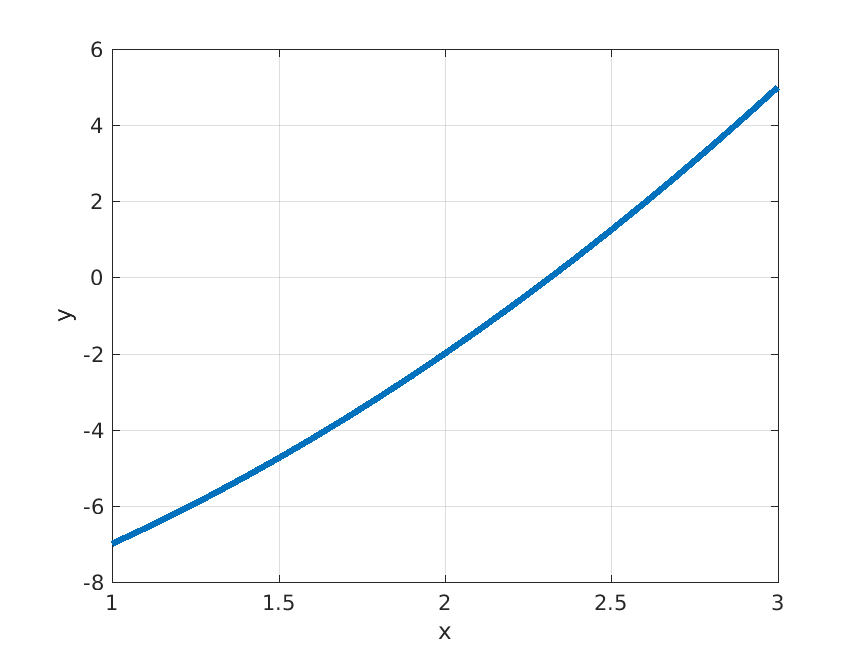
\includegraphics[scale=.4]{images/lecture1_fig3.png}
				\end{multicols}

				\btVFill
			\end{frame}
	
	% Section II
	\section{\sectionIItitle}\label{sectionII}

		% section II Outline
		\begin{frame}
			\large \textbf{Topic 2 - \sectionIItitle} \vspace{3mm}\\

			\begin{itemize}
				\item \hyperlink{sectionIIsubsectionI}{\sectionIIsubsectionItitle} \vspc %  section II subsection I
				\item \hyperlink{sectionIIsubsectionII}{\sectionIIsubsectionIItitle} \vspc % section II subsection II
				\item \hyperlink{sectionIIsubsectionIII}{\sectionIIsubsectionIIItitle} \vspc % section II subsection III
				\item \hyperlink{sectionIIsubsectionIV}{\sectionIIsubsectionIVtitle} \vspc % section II subsection IV
				\item \hyperlink{sectionIIsubsectionV}{\sectionIIsubsectionVtitle} \vspc % section II subsection V
				\item \hyperlink{sectionIIsubsectionVI}{\sectionIIsubsectionVItitle} \vspc % section II subsection VI
			\end{itemize}

		\end{frame}

		% section II subsection I
		\subsection{\sectionIIsubsectionItitle}\label{sectionIIsubsectionI}

			\begin{frame}[label=sectionIIsubsectionI]
				\frametitle{\sectionIIsubsectionItitle}
				\bigskip

				\btVFill
			\end{frame}

		% section II subsection II
		\subsection{\sectionIIsubsectionIItitle}\label{sectionIIsubsectionII}

			\begin{frame}
				\frametitle{\sectionIIsubsectionIItitle}
				\bigskip

				\btVFill 
			\end{frame}	

		% section II subsection III
		\subsection{\sectionIIsubsectionIIItitle}\label{sectionIIsubsectionIII}

			\begin{frame}
				\frametitle{\sectionIIsubsectionIIItitle}
				\bigskip

				\btVFill 
			\end{frame}

			\begin{frame}
				\frametitle{\sectionIIsubsectionIIItitle}
				\bigskip

				\btVFill 
			\end{frame}

			\begin{frame}
				\frametitle{\sectionIIsubsectionIIItitle}
				\bigskip
			
				\btVFill 
			\end{frame}

			\begin{frame}
				\frametitle{\sectionIIsubsectionIIItitle}
				\bigskip

				\btVFill 
			\end{frame}

		% section II subsection IV 
		\subsection{\sectionIIsubsectionIVtitle}\label{sectionIIsubsectionIV}

			\begin{frame}
				\frametitle{\sectionIIsubsectionIVtitle}
				\bigskip

				\btVFill 
			\end{frame}
		
	% Section III
	\section{\sectionIIItitle}\label{sectionIII}

		% section III Outline
		\begin{frame}
			\large \textbf{Topic 3 - \sectionIIItitle} \vspace{3mm}\\

			\begin{itemize}
				\item \hyperlink{sectionIIIsubsectionI}{\sectionIIIsubsectionItitle} \vspc %  section III subsection I
				\item \hyperlink{sectionIIIsubsectionII}{\sectionIIIsubsectionIItitle} \vspc % section III subsection II
				\item \hyperlink{sectionIIIsubsectionIII}{\sectionIIIsubsectionIIItitle} \vspc % section III subsection III
				%\item \hyperlink{sectionIIIsubsectionIV}{\sectionIIIsubsectionIVtitle} \vspc % section III subsection IV
			\end{itemize}

		\end{frame}

		% section III subsection I
		\subsection{\sectionIIIsubsectionItitle}\label{sectionIIIsubsectionI}

			\begin{frame}
				\frametitle{\sectionIIIsubsectionItitle}
				\bigskip
					
				\btVFill
			\end{frame}

			\begin{frame}
				\frametitle{\sectionIIIsubsectionItitle}
				\bigskip

				\btVFill
			\end{frame}

		% section III subsection II
		\subsection{\sectionIIIsubsectionIItitle}\label{sectionIIIsubsectionII}	

			\begin{frame}
				\frametitle{\sectionIIIsubsectionIItitle}
				\bigskip

				\btVFill
			\end{frame}

		% section III subsection III
		\subsection{\sectionIIIsubsectionIIItitle}\label{sectionIIIsubsectionIII}

			\begin{frame}
				\frametitle{\sectionIIIsubsectionIIItitle}
				\bigskip
				
				\btVFill
			\end{frame}

			\begin{frame}
				\frametitle{\sectionIIIsubsectionIIItitle}
				\bigskip
		
				\btVFill
			\end{frame}

			\begin{frame}
				\frametitle{\sectionIIIsubsectionIIItitle}
				\bigskip
				
				\btVFill
			\end{frame}

			\begin{frame}
				\frametitle{\sectionIIIsubsectionIIItitle}
				\bigskip

				\btVFill
			\end{frame}

			\begin{frame}
				\frametitle{\sectionIIIsubsectionIIItitle}
				\bigskip
				
				\btVFill
			\end{frame}

			\begin{frame}
				\frametitle{\sectionIIIsubsectionIIItitle}
				\bigskip
				
				\btVFill
			\end{frame}


	% Section IV
	\section{\sectionIVtitle}\label{sectionIV}

		% section IV Outline
		\begin{frame}
			\large \textbf{Topic 3 - \sectionIVtitle} \vspace{3mm}\\

			\begin{itemize}
				\item \hyperlink{sectionIVsubsectionI}{\sectionIVsubsectionItitle} \vspc %  section IV subsection I
				\item \hyperlink{sectionIVsubsectionII}{\sectionIVsubsectionIItitle} \vspc % section IV subsection II
				\item \hyperlink{sectionIVsubsectionIII}{\sectionIVsubsectionIIItitle} \vspc % section IV subsection III
				\item \hyperlink{sectionIVsubsectionIV}{\sectionIVsubsectionIVtitle} \vspc % section IV subsection IV
			\end{itemize}

		\end{frame}

		% section IV subsection I
		\subsection{\sectionIVsubsectionItitle}\label{sectionIVsubsectionI}

			\begin{frame}
				\frametitle{\sectionIVsubsectionItitle}
				\bigskip
					
				\btVFill
			\end{frame}

			\begin{frame}
				\frametitle{\sectionIVsubsectionItitle}
				\bigskip

				\btVFill
			\end{frame}


\end{document}





